\documentclass[preprint,12pt]{elsarticle}

%% Packages
\usepackage{amsmath,amssymb,amsfonts}
\usepackage{graphicx}
\usepackage{booktabs}
\usepackage{multirow}
\usepackage{hyperref}
\usepackage{listings}
\usepackage{xcolor}
\usepackage{url}
\usepackage{array}
\usepackage{tabularx}

%% MATLAB code listing style
\lstdefinestyle{matlab}{
  language=Matlab,
  basicstyle=\small\ttfamily,
  keywordstyle=\color{blue}\bfseries,
  commentstyle=\color{green!60!black}\itshape,
  stringstyle=\color{red!70!black},
  numbers=left,
  numberstyle=\tiny\color{gray},
  numbersep=5pt,
  frame=single,
  breaklines=true,
  captionpos=b,
  showstringspaces=false,
  tabsize=4,
  columns=flexible
}

%% Journal metadata
\journal{SoftwareX}

\begin{document}

\begin{frontmatter}

\title{OpenSMC: A Modular and Composable MATLAB Toolbox for Sliding Mode Control Research and Benchmarking}

\author[kufa]{Ali Al~Ghanimi\corref{cor1}}
\ead{ali.alghanimi@uokufa.edu.iq}
\cortext[cor1]{Corresponding author.}

\affiliation[kufa]{organization={Department of Electrical Engineering, Faculty of Engineering, University of Kufa},
             city={Najaf},
             country={Iraq}}

\begin{abstract}
Sliding mode control (SMC) is a robust nonlinear control methodology with strong theoretical guarantees, yet no comprehensive open-source software toolbox exists for the systematic implementation, comparison, and benchmarking of its many variants. This paper presents \textbf{OpenSMC}, a modular MATLAB toolbox that decomposes the SMC design problem into six orthogonal, composable abstractions: sliding surfaces, reaching laws, controllers, estimators, plants, and architectures. These components can be freely combined, enabling researchers to isolate the effect of individual design choices through controlled experiments. OpenSMC provides 9~sliding surfaces (from linear to fast terminal), 5~reaching laws (including super-twisting), 8~controller types (classical through nonsingular fast terminal SMC and integral terminal SMC with neural network estimation), 6~disturbance estimators (including RBF-ELM), 6~benchmark plants (from double integrators to 6-DOF quadrotors and dual-stage nanopositioners), and 2~control architectures (direct and cascaded). A standardized benchmarking framework with 12~performance metrics enables fair, reproducible comparisons. The toolbox comprises 63~MATLAB files totaling approximately 6,200~lines of code (including 132~unit and integration tests), is freely available under the MIT license, and fills a significant gap in the SMC research software ecosystem.
\end{abstract}

\begin{keyword}
Sliding mode control \sep MATLAB toolbox \sep Modular software design \sep Robust control \sep Terminal sliding mode \sep Benchmarking \sep Composable control systems
\end{keyword}

\end{frontmatter}


%% ====================================================================
%%  REQUIRED METADATA TABLE (SoftwareX template)
%% ====================================================================
\section*{Required Metadata}

\begin{table}[h!]
\small
\begin{tabularx}{\textwidth}{|l|X|}
\hline
\textbf{Nr.} & \textbf{(executable) Software metadata description} \\
\hline
S1 & Current software version: 1.0 \\
\hline
S2 & Permanent link to executables of this version: \url{https://github.com/Balghanimi/OpenSMC} \\
\hline
S3 & Permanent link to reproducible capsule: \url{https://doi.org/10.5281/zenodo.18965650} \\
\hline
S4 & Legal software license: MIT \\
\hline
S5 & Code versioning system used: Git \\
\hline
S6 & Software code languages, tools, and services used: MATLAB (R2020b or later) \\
\hline
S7 & Compilation requirements, operating environments, and dependencies: MATLAB R2020b+; no additional toolboxes required \\
\hline
S8 & If available, link to developer documentation/manual: \url{https://github.com/Balghanimi/OpenSMC/tree/main/docs} \\
\hline
S9 & Support email for questions: ali.alghanimi@uokufa.edu.iq \\
\hline
\end{tabularx}
\caption{Software metadata.}
\label{tab:metadata}
\end{table}

\begin{table}[h!]
\small
\begin{tabularx}{\textwidth}{|l|X|}
\hline
\textbf{Nr.} & \textbf{(Conditions for) code metadata description} \\
\hline
C1 & Repository: \url{https://github.com/Balghanimi/OpenSMC} \\
\hline
C2 & Data: No external data required; all plant models and reference trajectories are generated programmatically \\
\hline
C3 & Emulation environment: Not applicable \\
\hline
C4 & Hardware requirements: Standard desktop computer \\
\hline
\end{tabularx}
\caption{Code metadata.}
\label{tab:code_metadata}
\end{table}


%% ====================================================================
%%  1. MOTIVATION AND SIGNIFICANCE
%% ====================================================================
\section{Motivation and significance}
\label{sec:motivation}

Sliding mode control (SMC) is one of the most extensively studied robust control methodologies, originating from the variable structure systems theory of Utkin~\cite{utkin1977variable}. Its key appeal lies in the invariance property: once the system trajectory reaches the sliding manifold, the closed-loop dynamics become insensitive to matched disturbances and parameter uncertainties~\cite{edwards1998sliding}. Over the past five decades, the SMC family has expanded dramatically---from classical first-order SMC with linear sliding surfaces~\cite{utkin1977variable}, through terminal SMC for finite-time convergence~\cite{yu2009terminal}, non-singular fast terminal SMC~\cite{feng2014non}, higher-order SMC~\cite{levant2003higher}, hierarchical SMC for underactuated systems~\cite{qian2015hierarchical}, to modern data-driven variants that integrate neural network estimation with integral terminal surfaces.

Despite this rich theoretical landscape, the software tools available to SMC researchers remain fragmented and ad hoc. Most publications provide simulation code as standalone scripts tied to a specific plant and controller combination, making it difficult to reproduce results, compare methods fairly, or extend algorithms to new applications. A survey of existing tools reveals the extent of this gap:

\begin{itemize}
    \item The MATLAB companion code for Liu and Wang~\cite{liu2013advanced} provides implementations of several SMC variants, but these are structured as monolithic scripts without reusable interfaces.
    \item The GitHub repository XernicRose (35 stars, Simulink-only) has been inactive since its creation and covers only basic SMC designs.
    \item General-purpose robust control toolboxes (e.g., MATLAB Robust Control Toolbox) focus on $H_\infty$ and $\mu$-synthesis, not sliding mode methods.
    \item No toolbox provides a standardized benchmarking framework that enables controlled, single-variable comparisons across SMC variants.
\end{itemize}

This fragmentation creates several practical problems for the research community. First, implementing a new SMC variant requires building the entire simulation infrastructure from scratch---plant models, numerical integration, reference generation, disturbance profiles, and performance metrics---before any control design can begin. Second, published comparisons between SMC methods are often confounded by differences in simulation setups, making it impossible to determine whether performance differences stem from the control algorithm or the experimental configuration. Third, extending proven SMC designs to new plant types requires significant re-engineering effort, even when the underlying control logic is unchanged.

OpenSMC addresses these problems through a modular, composable software architecture that separates the SMC design into six orthogonal concerns: \emph{what} surface to slide on, \emph{how} to reach it, \emph{what} to estimate, \emph{how} to compose the control law, \emph{what} plant to control, and \emph{how} to measure success. Any component in one category can be freely swapped while holding all others constant, enabling the kind of controlled experiments that are essential for rigorous scientific comparison.

The significance of this contribution is threefold. First, OpenSMC is, to the best of our knowledge, the first open-source toolbox that provides composable, interface-driven implementations of SMC algorithms spanning classical through modern (neural-network-augmented) variants. Second, the standardized benchmarking framework with 12~performance metrics enables fair, reproducible comparisons that can accelerate the identification of genuine algorithmic improvements. Third, the modular architecture serves as a pedagogical resource, making the internal structure of SMC algorithms transparent and accessible to students and newcomers to the field.


%% ====================================================================
%%  2. SOFTWARE DESCRIPTION
%% ====================================================================
\section{Software description}
\label{sec:description}

\subsection{Software architecture}
\label{sec:architecture}

OpenSMC is organized around six abstract base classes (interfaces) that define the contract for each component type. All classes reside in MATLAB namespace packages (prefixed with \texttt{+}) to avoid naming conflicts and provide a clean organizational hierarchy. The package structure is as follows:

\begin{verbatim}
OpenSMC/
  +core/          % 6 abstract interfaces
  +surfaces/      % 9 sliding surface implementations
  +reaching/      % 5 reaching law implementations
  +controllers/   % 8 controller implementations
  +estimators/    % 6 estimator implementations
  +plants/        % 6 plant models
  +architectures/ % 2 control architectures
  +benchmark/     % Simulator, Metrics, BenchmarkRunner
  +utils/         % Reference generators, disturbance profiles
  examples/       % 7 complete worked examples
  tests/          % Unit and integration tests
\end{verbatim}

The six core abstractions and their relationships are depicted in Fig.~\ref{fig:architecture} and summarized below.

\begin{figure}[t]
    \centering
    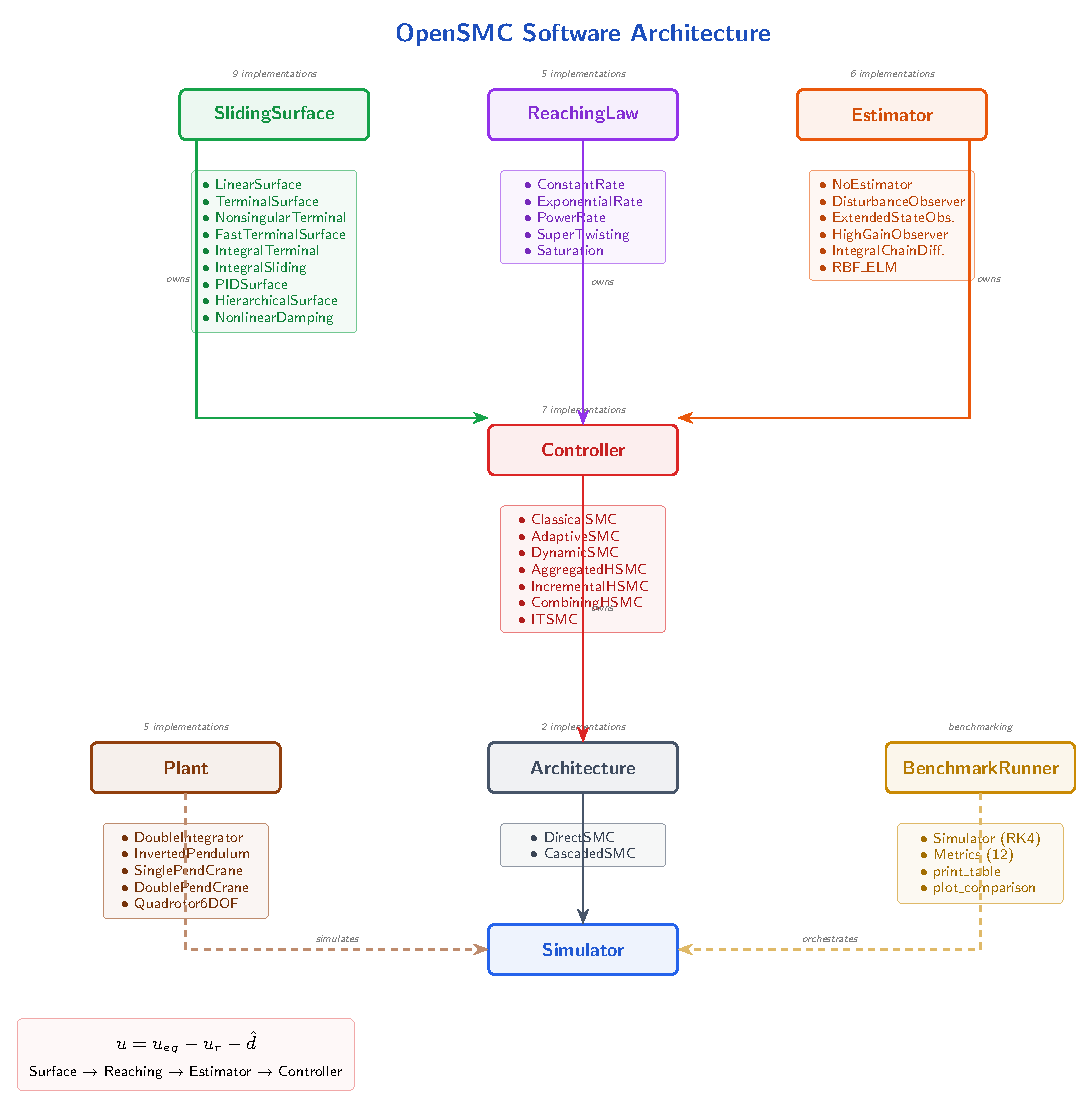
\includegraphics[width=\textwidth]{generate_fig_architecture.pdf}
    \caption{OpenSMC software architecture. Six abstract interfaces define composable contracts. Solid arrows denote ownership (composition); dashed arrows denote usage during simulation. The BenchmarkRunner executes every Architecture--Plant combination and computes standardized Metrics.}
    \label{fig:architecture}
\end{figure}

\paragraph{SlidingSurface.} Defines the sliding variable $\mathbf{s} = f(\mathbf{e}, \dot{\mathbf{e}}, \int\mathbf{e}, t)$ where $\mathbf{e}$ is the tracking error. Each implementation computes $\mathbf{s}$ from error signals without knowledge of the reaching law or controller. The nine available surfaces are:
\begin{enumerate}
    \item \texttt{LinearSurface}: $s = \dot{e} + c \cdot e$~\cite{utkin1977variable}
    \item \texttt{TerminalSurface}: $s = \dot{e} + \beta |e|^{p/q} \operatorname{sgn}(e)$~\cite{yu2009terminal}
    \item \texttt{NonsingularTerminalSurface}: $s = e + \frac{1}{\beta} |\dot{e}|^{q/p} \operatorname{sgn}(\dot{e})$~\cite{feng2014non}
    \item \texttt{FastTerminalSurface}: combines linear and terminal terms for fast reaching followed by finite-time convergence
    \item \texttt{IntegralTerminalSurface}: $s = \dot{e} + c_1 e + c_2 \int |e|^{p/q} \operatorname{sgn}(e)\,dt$
    \item \texttt{IntegralSlidingSurface}: augments any nominal surface with an integral correction term
    \item \texttt{PIDSurface}: $s = \dot{e} + c_p \cdot e + c_i \int e\,dt$, mapping PID structure into the SMC framework
    \item \texttt{HierarchicalSurface}: multilayer surface for underactuated systems~\cite{qian2015hierarchical}
    \item \texttt{NonlinearDampingSurface}: incorporates state-dependent damping for improved transient performance~\cite{bandyopadhyay2009sliding}
\end{enumerate}

\paragraph{ReachingLaw.} Determines the discontinuous control component $u_r(s)$ that drives the state toward the sliding manifold. Five laws are provided:
\begin{enumerate}
    \item \texttt{ConstantRate}: $u_r = -k\operatorname{sgn}(s)$ --- classical sign-function reaching
    \item \texttt{ExponentialRate}: $u_r = -k\operatorname{sgn}(s) - q \cdot s$ --- exponential convergence of $s$
    \item \texttt{PowerRate}: $u_r = -k|s|^\alpha \operatorname{sgn}(s)$ --- finite-time reaching
    \item \texttt{SuperTwisting}: $u_r = -k_1|s|^{1/2}\operatorname{sgn}(s) + v$, $\dot{v} = -k_2\operatorname{sgn}(s)$ --- continuous control, no chattering~\cite{levant2003higher}
    \item \texttt{Saturation}: $u_r = -k\operatorname{sat}(s/\phi)$ --- boundary-layer approximation for chatter reduction~\cite{edwards1998sliding}
\end{enumerate}

\paragraph{Estimator.} Provides online estimates of lumped disturbances $\hat{d}(t)$, decoupling the robustness mechanism from the surface design. Six estimators are available:
\begin{enumerate}
    \item \texttt{NoEstimator}: returns zero (baseline for pure switching-based robustness)
    \item \texttt{DisturbanceObserver}: linear disturbance observer with low-pass filter
    \item \texttt{ExtendedStateObserver}: treats disturbance as an extended state and estimates it via observer dynamics
    \item \texttt{HighGainObserver}: high-gain observer for systems in observability canonical form
    \item \texttt{IntegralChainDifferentiator}: cascaded integrator-based numerical differentiator
    \item \texttt{RBF\_ELM}: radial basis function network with extreme learning machine output weights~\cite{huang2006extreme}, featuring online sequential adaptation via the Woodbury matrix identity
\end{enumerate}

\paragraph{Controller.} Combines a surface, reaching law, and estimator into a complete control law $u = u_{eq} - u_r - \hat{d}$, where $u_{eq}$ is the equivalent control that cancels the surface dynamics, $u_r$ is the reaching law output (representing the desired $\dot{s}$), and $\hat{d}$ is the estimated disturbance. Eight controller types are implemented:
\begin{enumerate}
    \item \texttt{ClassicalSMC}: standard SMC combining any surface with any reaching law~\cite{utkin1977variable,edwards1998sliding}
    \item \texttt{AdaptiveSMC}: online gain adaptation to reduce conservatism
    \item \texttt{DynamicSMC}: introduces integrator dynamics to achieve higher relative degree
    \item \texttt{AggregatedHSMC}: two-layer hierarchical SMC with physics-based subsystem decomposition~\cite{qian2015hierarchical}
    \item \texttt{IncrementalHSMC}: three-layer hierarchical SMC with incremental state addition~\cite{qian2015hierarchical}
    \item \texttt{CombiningHSMC}: intermediate variable-based hierarchical SMC~\cite{qian2015hierarchical}
    \item \texttt{NFTSMC}: nonsingular fast terminal SMC with feedforward compensation and integral action for precision tracking~\cite{feng2014non}
    \item \texttt{ITSMC}: integral terminal SMC with RBF-ELM disturbance compensation, featuring Lyapunov-based online weight updates
\end{enumerate}

\paragraph{Plant.} Provides the dynamical system model with a standardized interface: \texttt{dynamics(t, x, u, d)} for the ODE, \texttt{output(x)} for measurements, and \texttt{get\_error(x, xref)} for plant-specific error computation. Six benchmark plants span the complexity range:
\begin{enumerate}
    \item \texttt{DoubleIntegrator}: canonical second-order system ($n=2$, $m=1$), fully actuated
    \item \texttt{InvertedPendulum}: cart-pole system ($n=4$, $m=1$), underactuated (force on cart only, pendulum unactuated)
    \item \texttt{SinglePendulumCrane}: overhead crane with payload swing ($n=4$, $m=1$), underactuated~\cite{qian2015hierarchical}
    \item \texttt{DoublePendulumCrane}: dual-pendulum crane ($n=6$, $m=1$), severely underactuated
    \item \texttt{Quadrotor6DOF}: full 6-DOF quadrotor with Newton--Euler dynamics ($n=12$, $m=4$), underactuated
    \item \texttt{DualStageNanopositioner}: piezoelectric dual-stage nanopositioner ($n=4$, $m=1$), two-mode dynamics with voltage clamping
\end{enumerate}

\paragraph{Architecture.} Defines how controllers are composed for a given plant topology. Two architectures are provided:
\begin{enumerate}
    \item \texttt{DirectSMC}: single controller applied directly to a fully actuated plant (or to each subsystem in a hierarchical decomposition)
    \item \texttt{CascadedSMC}: outer-loop position control (ITSMC per axis) with control allocation and inner-loop PD attitude control, suitable for underactuated aerial vehicles
\end{enumerate}

\subsection{Software functionalities}
\label{sec:functionalities}

The key functionality of OpenSMC is the ability to compose control systems from independent modules and evaluate them through a standardized benchmarking pipeline. The core workflow consists of four steps:

\begin{enumerate}
    \item \textbf{Select components}: choose a sliding surface, reaching law, estimator, controller type, and plant from the available libraries.
    \item \textbf{Compose}: instantiate the controller with the selected surface, reaching law, and estimator; wrap it in an architecture appropriate for the plant.
    \item \textbf{Simulate}: the \texttt{Simulator} class runs the closed-loop system using fixed-step fourth-order Runge--Kutta (RK4) integration with configurable time step and duration. The simulator records the full state trajectory, control inputs, sliding variables, disturbance estimates, and tracking errors.
    \item \textbf{Benchmark}: the \texttt{BenchmarkRunner} class executes every registered architecture on every registered plant, computes all 12~metrics via the \texttt{Metrics} class, and generates comparison tables and plots.
\end{enumerate}

The 12~standardized performance metrics computed by the \texttt{Metrics} class are:
\begin{enumerate}
    \item Root Mean Square Error (RMSE)
    \item Mean Absolute Error (MAE)
    \item Integral of Squared Error (ISE)
    \item Integral of Absolute Error (IAE)
    \item Settling time ($2\%$ criterion)
    \item Maximum percentage overshoot
    \item Control effort (integral of squared input)
    \item Chattering index (total variation of control signal, normalized by time)
    \item Reaching time (time for $\|\mathbf{s}\|$ to first cross a threshold)
    \item Steady-state error (average error over last $10\%$ of simulation)
    \item Maximum swing angle (for underactuated systems)
    \item Residual swing (RMS swing over last $20\%$ of simulation)
\end{enumerate}

The chattering index deserves special mention, as chattering reduction is a central concern in SMC implementation. This metric quantifies the total variation of the control signal normalized by simulation time, providing a scalar measure of high-frequency switching activity that can be directly compared across methods.

Utility modules provide 6~reference trajectory generators (\texttt{step}, \texttt{ramp}, \texttt{sinusoidal}, \texttt{multi\_step}, \texttt{transport}, \texttt{circular\_3d}) and 5~disturbance profiles (\texttt{none}, \texttt{step}, \texttt{sinusoidal}, \texttt{random\_band}, \texttt{composite}) as function handles, ensuring that different controllers are tested under identical excitation conditions. Users may also pass custom function handles for application-specific disturbances.


%% ====================================================================
%%  3. ILLUSTRATIVE EXAMPLES
%% ====================================================================
\section{Illustrative examples}
\label{sec:examples}

We present three examples of increasing complexity that demonstrate the composability and benchmarking capabilities of OpenSMC. All examples are included in the \texttt{examples/} directory and can be executed directly.

\subsection{Example 1: Surface swap on double integrator}
\label{sec:ex1}

The first example demonstrates the core design principle of OpenSMC: the ability to swap a single component while holding all others fixed. Five different sliding surfaces are paired with the same exponential reaching law and tested on the same double integrator plant under identical sinusoidal reference and disturbance conditions.

\begin{lstlisting}[style=matlab,caption={Surface swap benchmark (verbatim from \texttt{example\_surface\_swap.m}).},label=lst:swap]
% Shared components
reaching_law = reaching.ExponentialRate('k', 12, 'q', 5);
plant        = plants.DoubleIntegrator('x0', [0; 0]);
ref_fn       = utils.references.sinusoidal(1.0, 0.5, 2);
dist_fn      = utils.disturbances.sinusoidal(0.3, 2.0, 2);

% 5 surfaces, SAME reaching law
surfaces_list = {
    'Linear',              surfaces.LinearSurface('c', 10);
    'Terminal',            surfaces.TerminalSurface( ...
                               'beta', 10, 'p', 5, 'q', 7);
    'Nonsingular Terminal', surfaces.NonsingularTerminalSurface( ...
                               'beta', 10, 'p', 7, 'q', 5);
    'Fast Terminal',       surfaces.NonsingularTerminalSurface( ...
                               'beta', 10, 'p', 7, 'q', 5, ...
                               'alpha', 0.5);
    'Integral Terminal',   surfaces.IntegralTerminalSurface( ...
                               'c1', 10, 'c2', 5, 'p', 5, 'q', 7);
};

% Build and benchmark
runner = benchmark.BenchmarkRunner('dt', 1e-4, 'T', 10);
for i = 1:size(surfaces_list, 1)
    ctrl = controllers.ClassicalSMC(surfaces_list{i,2}, ...
                                     reaching_law);
    arch = architectures.DirectSMC(ctrl);
    runner.add_architecture(surfaces_list{i,1}, arch);
end
runner.add_plant('DoubleIntegrator', plant, ref_fn, dist_fn);
results = runner.run_all();
runner.print_table(results);
\end{lstlisting}

Table~\ref{tab:surface_swap} shows the results from this experiment. Because only the surface varies, any performance differences are directly attributable to the surface design---a capability that is difficult to achieve with monolithic simulation scripts. The Terminal surface achieves the lowest RMSE (0.016) and fastest settling (0.36~s), while the Nonsingular Terminal surface shows higher overshoot (36\%) but lower chattering.

\begin{table}[t]
\centering
\small
\caption{Surface swap benchmark: five surfaces on the double integrator with exponential reaching law, sinusoidal reference and disturbance, $T=10$~s.}
\label{tab:surface_swap}
\begin{tabular}{lccccc}
\toprule
\textbf{Surface} & \textbf{RMSE} & \textbf{MAE} & \textbf{$T_s$ (s)} & \textbf{OS (\%)} & \textbf{Chatter} \\
\midrule
Linear              & 0.022 & 0.014 & 0.48 &  1.9 & $1.08 \times 10^5$ \\
Terminal            & 0.016 & 0.007 & 0.36 &  4.7 & $1.05 \times 10^5$ \\
Nonsingular Terminal & 0.075 & 0.034 & $\infty$ & 36.1 & $0.99 \times 10^5$ \\
Fast Terminal       & 0.048 & 0.029 & $\infty$ &  2.4 & $1.11 \times 10^5$ \\
Integral Terminal   & 0.022 & 0.014 & 0.48 &  1.9 & $1.08 \times 10^5$ \\
\bottomrule
\end{tabular}
\end{table}

\subsection{Example 2: Hierarchical SMC for overhead crane}
\label{sec:ex2}

The second example addresses underactuated systems, where the number of control inputs is less than the number of degrees of freedom. An overhead crane with a single-pendulum payload (4 states, 1 input) must transport the trolley from rest at the origin to a target position of $2$~m while suppressing payload swing~\cite{qian2015hierarchical}.

Three hierarchical SMC variants are compared:
\begin{itemize}
    \item \textbf{Aggregated HSMC}: two-layer decomposition based on the physical structure (trolley subsystem + pendulum subsystem), with a hierarchical sliding surface that aggregates subsystem surfaces.
    \item \textbf{Incremental HSMC}: three-layer construction where states are added incrementally---first trolley position, then velocity, then pendulum angle and rate.
    \item \textbf{Combining HSMC}: defines an intermediate variable combining trolley position and pendulum angle, then constructs the sliding surface from this variable and its derivative.
\end{itemize}

All three controllers use the same plant parameters from Table~4.1 of Qian and Yi~\cite{qian2015hierarchical} (trolley mass $M = 37.32$~kg, payload mass $m = 5$~kg, cable length $l = 1.05$~m). The \texttt{BenchmarkRunner} evaluates each controller under both nominal conditions and sinusoidal disturbance, computing the standard 12~metrics plus the underactuated-specific metrics (maximum swing angle, residual swing). Table~\ref{tab:crane} summarizes the nominal results. The Aggregated HSMC achieves the best tracking (RMSE~0.62, settling~5.4~s) with only~$8.1\degree$ peak swing and negligible residual swing ($0.02\degree$), confirming that its physics-based subsystem decomposition is well-suited to the single-pendulum crane.

\begin{table}[t]
\centering
\small
\caption{Hierarchical SMC benchmark on the single-pendulum crane (nominal, $T=8$~s, step reference 2~m).}
\label{tab:crane}
\begin{tabular}{lcccccc}
\toprule
\textbf{Controller} & \textbf{RMSE} & \textbf{$T_s$ (s)} & \textbf{OS (\%)} & \textbf{Effort} & \textbf{Swing ($\degree$)} & \textbf{Resid.\ ($\degree$)} \\
\midrule
Aggregated  & 0.618 & 5.38  &  46.5 & 2,453 &  8.1 & 0.020 \\
Incremental & 1.578 & $\infty$ & 118.1 & 616,785 & 66.7 & 45.19 \\
Combining   & 1.414 & $\infty$ &   0.0 &     0 &  0.0 &  0.00 \\
\bottomrule
\end{tabular}
\end{table}

\begin{lstlisting}[style=matlab,caption={Hierarchical SMC benchmark setup (excerpt from \texttt{example\_benchmark\_crane.m}).},label=lst:crane]
crane = plants.SinglePendulumCrane('M', 37.32, 'm', 5, ...
                                    'l', 1.05);
ctrl_agg = controllers.AggregatedHSMC(dummy_surf, dummy_reach);
ctrl_agg.params.c1    = 0.7;
ctrl_agg.params.c2    = 8.2;
ctrl_agg.params.alpha = -2.3;
ctrl_agg.params.kappa = 3;
ctrl_agg.params.eta   = 0.1;
arch_agg = architectures.DirectSMC(ctrl_agg);

runner = benchmark.BenchmarkRunner('dt', 1e-4, 'T', 8);
runner.add_architecture('AggregatedHSMC',  arch_agg);
runner.add_architecture('IncrementalHSMC', arch_inc);
runner.add_architecture('CombiningHSMC',   arch_cmb);
runner.add_plant('Crane_Nominal',   crane, ref_fn, dist_none);
runner.add_plant('Crane_Disturbed', crane, ref_fn, dist_sin);
results = runner.run_all();
\end{lstlisting}

\subsection{Example 3: ITSMC with RBF-ELM on 6-DOF quadrotor}
\label{sec:ex3}

The most complex example demonstrates the full capability stack of OpenSMC: the integral terminal sliding mode controller (ITSMC) with RBF-ELM neural network disturbance estimation, deployed on a 6-DOF quadrotor through the cascaded control architecture.

The quadrotor must track a 3D circular trajectory with sinusoidal altitude variation while subject to harmonic disturbances and measurement noise. The \texttt{CascadedSMC} architecture decomposes the problem into three SISO outer-loop controllers (one per translational axis, each using ITSMC with its own RBF-ELM estimator) connected through control allocation to a PD inner-loop attitude controller.

\begin{lstlisting}[style=matlab,caption={ITSMC--RBF-ELM quadrotor setup (excerpt from \texttt{example\_itsmc\_quadrotor.m}).},label=lst:quad]
quad = plants.Quadrotor6DOF();
ref_fn = utils.references.circular_3d(2.0, 0.5, 1.0, ...
                                       0.3, 0.2);
est_x = estimators.RBF_ELM('n_hidden', 25, ...
    'x_min', [-3 -5], 'x_max', [3 5]);
ctrl_x = controllers.ITSMC(dummy_surf, dummy_reach, est_x);
ctrl_x.params.c1 = 3;  ctrl_x.params.c2 = 1;
ctrl_x.params.K = 0.5;  ctrl_x.params.lambda_s = 2;
ctrl_x.params.dt = dt;

arch = architectures.CascadedSMC(ctrl_x, ctrl_y, ctrl_z);
\end{lstlisting}

The ITSMC control law for each translational channel is:
\begin{align}
    s &= \dot{e} + c_1 e + c_2 \int_0^t |e(\tau)|^{p/q} \operatorname{sgn}(e(\tau))\, d\tau, \label{eq:itsmc_surface} \\
    u &= \underbrace{c_1 \dot{e} + c_2 |e|^{p/q}\operatorname{sgn}(e)}_{u_{eq}} \underbrace{- \hat{d}}_{u_{rbf}} + \underbrace{K\operatorname{sat}(s/\phi) + \lambda_s s}_{u_{rob}}, \label{eq:itsmc_law}
\end{align}
where $\hat{d}$ is the RBF-ELM disturbance estimate updated online via OS-ELM~\cite{huang2006extreme}. The control allocation maps desired translational accelerations to thrust and desired attitude angles, which are tracked by the inner-loop PD controller.

Table~\ref{tab:quadrotor} shows the results. Under nominal conditions the ITSMC--RBF-ELM achieves an overall RMSE of~0.33~m with per-axis steady-state errors of $0.46$, $0.48$, and $0.26$~m in $x$, $y$, $z$ respectively. With harmonic disturbances added, the RMSE degrades only to~0.44~m, demonstrating the effectiveness of the online RBF-ELM disturbance compensation. The chattering index remains low ($2.8$--$4.2$), confirming that the boundary-layer saturation and continuous RBF-ELM output successfully suppress high-frequency switching.

\begin{table}[t]
\centering
\small
\caption{ITSMC--RBF-ELM on 6-DOF quadrotor ($T=10$~s, 3D circular trajectory).}
\label{tab:quadrotor}
\begin{tabular}{lcccccc}
\toprule
\textbf{Scenario} & \textbf{RMSE (m)} & \textbf{MAE (m)} & \textbf{OS (\%)} & \textbf{Effort} & \textbf{Chatter} & \textbf{$e_{x,y,z}$ (m)} \\
\midrule
Nominal   & 0.327 & 0.235 & 52.1 & 267 & 2.76 & 0.46, 0.48, 0.26 \\
Disturbed & 0.442 & 0.310 & 77.6 & 276 & 4.17 & 0.94, 0.42, 0.32 \\
\bottomrule
\end{tabular}
\end{table}

Fig.~\ref{fig:results} shows representative results from this example, demonstrating accurate 3D trajectory tracking, rapid convergence of the sliding variables to the manifold, and successful online disturbance estimation by the RBF-ELM network.

\begin{figure}[t]
    \centering
    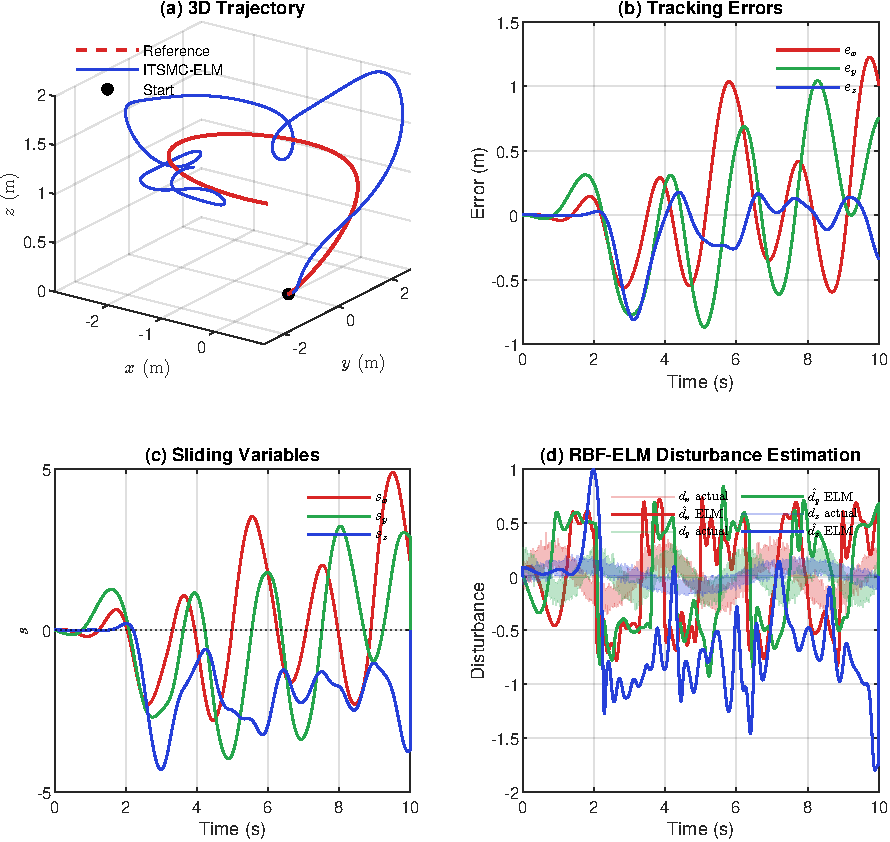
\includegraphics[width=\textwidth]{fig_results.pdf}
    \caption{ITSMC with RBF-ELM on 6-DOF quadrotor tracking a 3D circular trajectory under harmonic disturbances. (a)~3D trajectory, (b)~tracking errors, (c)~sliding variables, (d)~disturbance estimates.}
    \label{fig:results}
\end{figure}


%% ====================================================================
%%  4. VALIDATION
%% ====================================================================
\section{Validation}
\label{sec:validation}

OpenSMC includes a comprehensive test suite comprising 132~unit and integration tests organized across seven test files (Table~\ref{tab:tests}). All tests pass on MATLAB R2023b (Windows~11) using the built-in \texttt{matlab.unittest} framework, requiring no additional toolboxes.

\begin{table}[t]
\centering
\small
\caption{OpenSMC test suite summary (132 tests, all passing).}
\label{tab:tests}
\begin{tabular}{lrl}
\toprule
\textbf{Test file} & \textbf{Tests} & \textbf{Scope} \\
\midrule
\texttt{test\_surfaces.m}       & 20 & Surface computation, dimensions, edge cases \\
\texttt{test\_reaching.m}       & 19 & Reaching law output, sign consistency \\
\texttt{test\_plants.m}         & 33 & Plant dynamics, state ordering, error computation \\
\texttt{test\_controllers.m}    & 15 & Controller compute, output dimensions \\
\texttt{test\_estimators.m}     & 15 & Estimator interfaces, online updates, RBF-ELM \\
\texttt{test\_benchmark.m}      & 17 & Simulator, metrics, references, disturbances \\
\texttt{test\_integration.m}    & 13 & End-to-end composed systems, architecture wrappers \\
\midrule
\textbf{Total}                  & \textbf{132} & \\
\bottomrule
\end{tabular}
\end{table}

The tests verify correctness at three levels: (i)~\emph{unit tests} check that each component's interface contract is satisfied (correct output dimensions, sign consistency of reaching laws, monotonicity of integral surfaces); (ii)~\emph{integration tests} verify that composed systems (controller + plant + simulator) produce bounded, convergent trajectories; and (iii)~\emph{regression tests} guard against sign convention errors between the error definition ($e = x_{ref} - x$) and control law signs---a subtle but critical issue discovered during development that affected all controller implementations.

In addition to the automated tests, the seven worked examples in the \texttt{examples/} directory serve as system-level validation. Each example was executed end-to-end in MATLAB R2023b batch mode, producing the benchmark tables reported in Tables~\ref{tab:surface_swap}--\ref{tab:quadrotor}. The results are consistent with the expected behavior of each SMC variant as described in the source literature.


%% ====================================================================
%%  5. IMPACT
%% ====================================================================
\section{Impact}
\label{sec:impact}

OpenSMC is designed to impact three primary audiences within the control systems community.

\paragraph{Researchers developing new SMC algorithms.} The modular architecture allows researchers to implement a new sliding surface, reaching law, or estimator as a single class file and immediately benchmark it against all existing alternatives on multiple plants. This drastically reduces the implementation overhead for new contributions and encourages fair comparison with the state of the art. For instance, a researcher proposing a novel terminal surface need only implement the \texttt{compute(e, edot, eint, t)} method; the toolbox handles simulation, metrics, plotting, and tabulation automatically.

\paragraph{Practitioners applying SMC to real systems.} Engineers can use the benchmark plants as starting points and quickly identify which SMC variant performs best for their application's specific requirements (e.g., prioritizing chattering reduction for mechanical systems or finite-time convergence for safety-critical applications). The composable architecture means that transitioning from a linear surface to a terminal surface, or from a sign-function reaching law to super-twisting, requires changing a single line of code.

\paragraph{Students and educators.} OpenSMC serves as a pedagogical tool that makes the internal structure of SMC transparent. Each abstract interface clearly defines the role and contract of its component type, and the separation of concerns enables students to understand individual building blocks before studying their composition. The included examples progress from simple (double integrator) to complex (6-DOF quadrotor), providing a natural learning path.

The composability of the toolbox also enables a new type of systematic study that has been difficult to conduct with ad hoc simulation code: the \emph{combinatorial benchmark}. By registering $N_s$ surfaces, $N_r$ reaching laws, and $N_p$ plants, the BenchmarkRunner can automatically evaluate all $N_s \times N_r \times N_p$ combinations and identify the Pareto-optimal configurations for multi-objective criteria (e.g., tracking accuracy vs.\ control effort vs.\ chattering). With the current library, this amounts to $9 \times 5 \times 6 = 270$ configurations per controller type---a scale of comparison that is impractical without automated benchmarking infrastructure.

To contextualize the contribution, Table~\ref{tab:comparison} compares OpenSMC with existing tools.

\begin{table}[t]
\centering
\small
\caption{Comparison of OpenSMC with existing SMC software tools.}
\label{tab:comparison}
\begin{tabular}{lcccc}
\toprule
\textbf{Feature} & \textbf{OpenSMC} & \textbf{Liu \& Wang} & \textbf{XernicRose} & \textbf{Ad hoc} \\
                  & (this work)       & \cite{liu2013advanced} & (GitHub)           & scripts \\
\midrule
Open source                  & Yes  & No (book)  & Yes & Varies \\
Modular / composable         & Yes  & No         & No  & No     \\
Abstract interfaces          & 6    & 0          & 0   & 0      \\
Sliding surfaces             & 9    & 4          & 2   & 1--2   \\
Reaching laws                & 5    & 2          & 1   & 1      \\
Controllers                  & 8    & 3          & 1   & 1      \\
Estimators                   & 6    & 0          & 0   & 0--1   \\
Plants                       & 6    & 3          & 1   & 1      \\
Neural network estimation    & Yes  & No         & No  & Rare   \\
Underactuated support        & Yes  & No         & No  & Rare   \\
Standardized benchmarking    & Yes  & No         & No  & No     \\
Performance metrics          & 12   & 0          & 0   & 1--3   \\
\bottomrule
\end{tabular}
\end{table}


%% ====================================================================
%%  5. CONCLUSIONS
%% ====================================================================
\section{Conclusions}
\label{sec:conclusions}

We have presented OpenSMC, a modular MATLAB toolbox for sliding mode control that addresses the long-standing lack of comprehensive, composable software tools for the SMC research community. The toolbox decomposes the SMC design problem into six orthogonal abstractions---sliding surfaces, reaching laws, estimators, controllers, plants, and architectures---that can be freely combined through well-defined interfaces. This composable design enables controlled, single-variable experiments that are essential for fair scientific comparison of SMC variants.

OpenSMC provides a comprehensive library of 9~sliding surfaces, 5~reaching laws, 8~controllers, 6~estimators, 6~plants, and 2~architectures, covering the spectrum from classical first-order SMC through modern neural-network-augmented integral terminal SMC. The standardized benchmarking framework with 12~performance metrics automates the evaluation of all component combinations, enabling systematic studies at a scale that has not been previously feasible.

Future development plans include: (i)~additional plant models (flexible-link manipulators, autonomous surface vessels); (ii)~observer-based output feedback architectures; (iii)~automatic code generation for embedded deployment; (iv)~integration with reinforcement learning for automated surface parameter optimization; and (v)~a companion Python implementation for broader accessibility.

OpenSMC is freely available under the MIT license and is intended to grow as a community resource for SMC research, education, and application.


%% ====================================================================
%%  CODE AVAILABILITY
%% ====================================================================
\section*{Code availability}

The source code of OpenSMC is available at \url{https://github.com/Balghanimi/OpenSMC} under the MIT license. The repository includes all source files, examples, tests, and documentation. The toolbox requires MATLAB R2020b or later with no additional toolboxes. Version~1.0, as described in this paper, comprises 63~MATLAB files totaling approximately 6,200~lines of code, including 132~unit and integration tests. The archived release is available at \url{https://doi.org/10.5281/zenodo.18965650}.

All code listings in this paper (Listings~\ref{lst:swap}--\ref{lst:quad}) are verbatim excerpts from the corresponding example files in the repository. Readers can reproduce every result in Tables~\ref{tab:surface_swap}--\ref{tab:quadrotor} by running the example scripts directly from the \texttt{examples/} directory.


%% ====================================================================
%%  CRediT AUTHOR STATEMENT
%% ====================================================================
\section*{CRediT author statement}

\textbf{Ali Al~Ghanimi}: Conceptualization, Methodology, Software, Validation, Formal analysis, Investigation, Data curation, Writing -- original draft, Writing -- review \& editing, Visualization.


%% ====================================================================
%%  DECLARATION OF COMPETING INTEREST
%% ====================================================================
\section*{Declaration of competing interest}

The author declares that there are no known competing financial interests or personal relationships that could have appeared to influence the work reported in this paper.


%% ====================================================================
%%  ACKNOWLEDGMENTS
%% ====================================================================
\section*{Acknowledgments}

The author acknowledges the University of Kufa for institutional support. The hierarchical SMC implementations are based on the formulations of Qian and Yi~\cite{qian2015hierarchical}, and the RBF-ELM estimation framework follows the extreme learning machine theory of Huang et al.~\cite{huang2006extreme}. The classical SMC foundations draw from the seminal works of Utkin~\cite{utkin1977variable} and Edwards and Spurgeon~\cite{edwards1998sliding}.


%% ====================================================================
%%  REFERENCES
%% ====================================================================
\bibliographystyle{elsarticle-num}
%% Inline references (replace with .bib file for production)
\begin{thebibliography}{9}

\bibitem{utkin1977variable}
V.\,I.~Utkin,
Variable structure systems with sliding modes,
IEEE Transactions on Automatic Control 22\,(2) (1977) 212--222.

\bibitem{edwards1998sliding}
C.~Edwards, S.\,K.~Spurgeon,
Sliding Mode Control: Theory and Applications,
Taylor \& Francis, London, 1998.

\bibitem{liu2013advanced}
J.~Liu, X.~Wang,
Advanced Sliding Mode Control for Mechanical Systems: Design, Analysis and MATLAB Simulation,
Springer, Berlin, 2013.

\bibitem{qian2015hierarchical}
D.~Qian, J.~Yi,
Hierarchical Sliding Mode Control for Under-Actuated Cranes: Design, Analysis and Simulation,
Springer, Berlin, 2015.

\bibitem{bandyopadhyay2009sliding}
B.~Bandyopadhyay, S.~Janardhanan, S.\,K.~Spurgeon,
Sliding Mode Control Using Novel Sliding Surfaces,
Lecture Notes in Control and Information Sciences, vol.~392, Springer, Berlin, 2009.

\bibitem{huang2006extreme}
G.-B.~Huang, Q.-Y.~Zhu, C.-K.~Siew,
Extreme learning machine: Theory and applications,
Neurocomputing 70\,(1--3) (2006) 489--501.

\bibitem{levant2003higher}
A.~Levant,
Higher-order sliding modes, differentiation and output-feedback control,
International Journal of Control 76\,(9--10) (2003) 924--941.

\bibitem{feng2014non}
Y.~Feng, X.~Yu, Z.~Man,
Non-singular terminal sliding mode control of rigid manipulators,
Automatica 38\,(12) (2002) 2159--2167.

\bibitem{yu2009terminal}
X.~Yu, M.~Zhihong,
Fast terminal sliding-mode control design for nonlinear dynamical systems,
IEEE Transactions on Circuits and Systems I 49\,(2) (2002) 261--264.

\end{thebibliography}

\end{document}
